\section{Background}
\subsection{Literature Review}
Highly up to date review of NF blast loading. 
Andys recent work. 
Shins work (and with Cormie report).
\subsection{Scaling laws}
Certain parameters can be scaled via Hopkinson-Cranz (or `cube-root') scaling, proposed independently by \textcite{hopkinsonBoardMinutes1915} and  \textcite{cranzLehrbuchBallistik1926}, in order to provide a method of comparison in blast scenarios.
This states similarity exists between blast waves produced at identical scaled distances from two explosive charges of the same geometry but different masses.
Therefore, the blast pressure generated at a distance R (stand-off) from an explosive mass W will be similar to the blast pressure created at a distance KR from a mass of K$^3$W.

This concept of \textit{scaled distance, Z}, with units m/kg$^{1/3}$, is expressed as:
\begin{equation}
Z=\frac{R}{W^{1/3}}
\end{equation}
TNT equivalence in kilograms is used as a universal unit here with regard to explosive charges \parencite{cormieBlastEffectsBuildings2009}.
\begin{figure}%[h]
	\includegraphics[width=0.85\textwidth, keepaspectratio=true]{Vec_Graphics/Hop_Cranz_Scaling}
	\centering
	\caption{Hopkinson-Cranz blast wave scaling}
	\label{fig:Hop_Cranz_Scaling}
\end{figure}
Due to scaling, a specific blast parameter measured at a scaled distance from a target can be used as a reference for determining the same parameter for a charge at an equal scaled distance but different combination of charge mass and stand-off.

In Hopkinson-Cranz scaling, pressures are identical between scaled and actual values, and all times are scaled by the same value as the length scale factor, K, or the cube-root of the charge mass \parencite{kinneyExplosiveShocksAir1985}.
To summarise:
\begin{equation*}
\begin{aligned}
 p_{actual} &= p_{scaled} 
\\ 	 t_{actual} &= t_{scaled}W^{1/3} 
\\	 \text{and } i_{actual} &= i_{scaled}W^{1/3}. 
\end{aligned}
\end{equation*}

\subsection{Empirical / semi - empirical predictive methods in blast engineering}
The most prevalent predictive method in blast engineering is the ConWep computer code \parencite{hydeConventionalWeaponsEffect1991} that utilises the \textcite{kingeryAirblastParametersTNT} predictions (abbreviated as KB henceforth).
The KB method ``look-up" method relies on curves fit to a compilation of data from both computer analyses and experimental measurements.
It allows the prediction of pressure, impulse, arrival time and duration to be determined for scaled distance, Z, between 0.067 and 39.67 m/kg$^{1/3}$. 
The smaller scaled distances are mainly derived from computer analyses due to difficulty measuring the extremely high pressures close to the explosive source \parencite{esparzaBlastMeasurementsEquivalency1986}.
This allows for rapid evaluation of blast wave parameters from a given explosive event. 
A comprehensive review of current methods for predicting blast wave parameters is given by \textcite{remennikovReviewMethodsPredicting2003}. 

These methods are unsuitable, however, when considering explosives located extremely close to a structure, where complex interactions between the explosive and target result in a highly spatially non-uniform loading and do not give the user any insight into the distribution of this loading. 



\subsection{Predictive approaches of blast wave parameters in urban environments}
Considering predictive methods of blast loading on a larger scale, particularly in city geometries, brings forth issues of complex wave interactions.  
\textcite{remennikovModellingBlastLoads2005} present a framework to determine load enhancement factors from adjacent buildings in urban terrain, as they mention actual blast loads can be significantly greater or lesser than simple predictions due to shadowing or confinement respectively if these adjacent buildings are not factored into consideration. 

For simple geometries and city streets, empirical rules can be formulated to predict blast resultants on building facades; as complexity of city street layouts increase, such rules become more difficult to develop and more complex analyses are recommended \parencite{smithBlastWavePropagation2006}.
Extending this analysis \textcite{remennikovPredictionAirblastLoads2012} use ANNs to predict blast loads in more complex city street environments, where street configuration parameters were the principle inputs and peak pressures and impulses were the outputs. 
 
\textcite{remennikovPredictingEffectivenessBlast2007} use an ANN to accurately predict the blast environment (peak overpressure and peak scaled impulse) behind a vertical wall barrier for various blast wall scenarios. 
To train and validate the ANN, the authors develop a database through a series of measurements of the blast environment behind the barrier. 
The principal parameters controlling the blast environment, such as wall height, distance behind the wall, height above ground, and standoff distance are used as the training input data.
From this data the authors develop contour plots of overpressure and impulse adjustment factors to simplify predicting the effectiveness of blast barriers.

\textcite{floodModelingBlastWave2009} also replicate this blast wall scenario and extend the analyses in a few ways. 
The authors firstly sample in the time domain which enables the ANN to predict pressure peaks and allows the user to understand the time-wise progress of the blast wave over critical surfaces.
In this instance, the output from the ANN are estimates of the peaks in the pressure wave, the arrival time of these peaks and their decay rates.
The authors finally propose a concept of course-grain modelling, previously shown to work in modelling dynamic heat transfer in buildings \parencite{floodSimulatingThermalBehavior2004}. 
This concept is similar to traditional computational fluid dynamics or finite element analyses in that the environment is discretized and the state of each element advances in time, the difference being that no physical equations are solved at each time step; a trained ANN instead implements the output of these physical equations \parencite{floodRapidSimulationBlast2012}.

One approach identified for simplifying the challenge of blast load prediction is to use ray tracing algorithms (specifically shortest path ray tracing). 
Ray tracing methods search for the shortest path a wave can follow from the point of detonation to any target points, considering reflection and diffraction and has been implemented by \textcite{frankFastRunningModel2008} to produce a fast running tool to calculate air blast pressure waveforms in urban environments. However, although a promising methodology this tool does not provide accurate enough solutions to be used reliably by blast protection engineers. 

An alternative approach to simplifying the challenge lies in considering the trade-off between mesh resolution, computational time and accuracy.
\textcite{frankComparisonFastRunning2008} compare their proposed fast running model (with ray tracing) with a coarse mesh finite element code \parencite{lohnerFiniteElementFluxcorrected1987} where they state reasonable solutions are provided, however, more accuracy is certainly required to be used in civil engineering applications.

\textcite{lohnerComparisonCoarseFine2004} argue that coarse CFD simulations can provide a much higher accuracy than line-of-site (ray tracing style) calculations, particularly in more complex geometries that entail more complex wave interactions.  
The authors provide some guidance on necessary requirements of running these coarse CFD simulations and provide three important conclusions: peak impulses are adequately captured in coarse meshes, peak pressures show discrepancies between $25-50\%$ between coarse and fine meshes and finally coarse grids do not capture weaker shock reflections between buildings. 

\textcite{klomfassAccuracyCFDPredictions2018} perform a similar set of analyses, with the intention, however, of investigating the discretisation error associated with the finite spatial resolution (similar to the course-grain methodology proposed by \textcite{floodRapidSimulationBlast2012}). 
An important conclusion from this work finds a similar conclusion to \textcite{lohnerComparisonCoarseFine2004} in that maximum impulse does not need an error correction, but it also concludes that practically useful predictions of maximum overpressures can be obtained on a standard computer within a few minutes provided the discretisation error is considered and suggests a very promising area of further research. 

